\chapter{Mathematical Background}
\section{Systems of Linear equations}

Consider a system of two linear equations with two unknowns:
\begin{align}
    2x - y &= 0 \\
    -x + 2y &= 3
\end{align}

This system can be represented in matrix form as:
\begin{equation*}
    \begin{bmatrix}
        2 & -1 \\
        -1 & 2
    \end{bmatrix}
    \begin{bmatrix}
        x \\
        y
    \end{bmatrix}
    =
    \begin{bmatrix}
        0 \\
        3
    \end{bmatrix}
\end{equation*}
where the matrix on the left is the coefficient matrix, and the vector on the right is the vector of constants.

\subsection*{Graphical Interpretation}

Each equation in the system corresponds to a straight line in the 2D plane, and the solution of the system is the intersection point of these lines.

\begin{center}
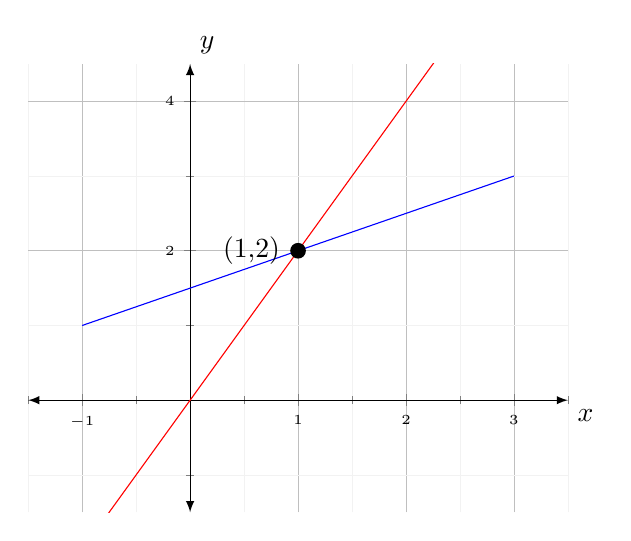
\begin{tikzpicture}
\begin{axis}[
    xlabel={$x$},
    ylabel={$y$},
    xmin=-1, xmax=3,
    ymin=-1, ymax=4,
    grid=both,
    grid style={line width=.1pt, draw=gray!10},
    major grid style={line width=.2pt,draw=gray!50},
    axis lines=middle,
    minor tick num=1,
    enlargelimits={abs=0.5},
    axis line style={latex-latex},
    ticklabel style={font=\tiny},
    xlabel style={at={(ticklabel* cs:1)},anchor=north west},
    ylabel style={at={(ticklabel* cs:1)},anchor=south west}
]

% Lines
\addplot[domain=-1:3, samples=2, red]{2*x};
\addplot[domain=-1:3, samples=2, blue]{(x+3)/2};
% Solution point
\node[label={180:{(1,2)}},circle,fill,inner sep=2pt] at (axis cs:1,2) {};
\end{axis}
\end{tikzpicture}
\end{center}

This graphical representation is known as the \textbf{Row Formulation} of the system.

\subsection*{Column Formulation}

Alternatively, we can express the system in terms of a linear combination of column vectors, known as the \textbf{Column Formulation}.

\begin{equation*}
    x\begin{bmatrix}
        2 \\
        -1
    \end{bmatrix}
    +
    y\begin{bmatrix}
        -1 \\
        2
    \end{bmatrix}
    =
    \begin{bmatrix}
        0 \\
        3
    \end{bmatrix}
\end{equation*}

The weights \( x \) and \( y \) are the scalars that, when used to multiply the respective column vectors and then added together, yield the resultant vector on the right-hand side.

% \subsection*{Geometrical Interpretation}

% The solution \( (x = 1, y = 2) \) represents the point at which the linear combination of the column vectors equals the constant vector:
% \begin{equation*}
%     1\begin{bmatrix}
%         2 \\
%         -1
%     \end{bmatrix}
%     +
%     2\begin{bmatrix}
%         -1 \\
%         2
%     \end{bmatrix}
%     =
%     \begin{bmatrix}
%         0 \\
%         3
%     \end{bmatrix}
% \end{equation*}

% The collection of all possible linear combinations of the column vectors spans the entire 2D plane, which in linear algebra is referred to as the \textbf{span} of the vectors.

\subsection*{Geometrical Representation}

The solution to the system of equations corresponds to the specific linear combination of the column vectors that results in the right-hand side vector.

% The column vectors diagram
\begin{center}
\begin{tikzpicture}
\begin{axis}[
    axis lines=middle,
    xlabel={$x$},
    ylabel={$y$},
    xmin=-3, xmax=3,
    ymin=-3, ymax=4,
    grid=major,
    grid style=dashed,
]

% Vector [2 -1]
\addplot[->, thick, blue] coordinates {(0,0) (2,-1)};
\node[anchor=south] at (axis cs:1,-0.5) {$\begin{bmatrix} 2 \\ -1 \end{bmatrix}$};

% Vector [-1 2]
\addplot[->, thick, red] coordinates {(0,0) (-1,2)};
\node[anchor=west] at (axis cs:-1,1) {$\begin{bmatrix} -1 \\ 2 \end{bmatrix}$};

% Resultant vector [0 3]
\addplot[->, thick, green] coordinates {(0,0) (0,3)};
\node[anchor=west] at (axis cs:0,1.5) {$\begin{bmatrix} 0 \\ 3 \end{bmatrix}$};

\end{axis}
\end{tikzpicture}
\end{center}

The combination of \( x = 1 \) and \( y = 2 \) yields the solution to the system:
\[
1 \begin{bmatrix} 2 \\ -1 \end{bmatrix} + 2 \begin{bmatrix} -1 \\ 2 \end{bmatrix} = \begin{bmatrix} 0 \\ 3 \end{bmatrix}
\]

\begin{center}
\begin{tikzpicture}
\begin{axis}[
    axis lines=middle,
    xlabel={$x$},
    ylabel={$y$},
    xmin=-3, xmax=3,
    ymin=-3, ymax=4,
    grid=major,
    grid style=dashed,
]

% Vector [2 -1]
\addplot[->, thick, blue] coordinates {(0,0) (2,-1)};
\node[anchor=south] at (axis cs:1,-2) {$\begin{bmatrix} 2 \\ -1 \end{bmatrix}$};

% Vector [-1 2]
\addplot[->, thick, red] coordinates {(2,-1) (1,1)};
\node[anchor=west] at (axis cs:1,2) {$2\begin{bmatrix} -1 \\ 2 \end{bmatrix}$};

\addplot[->, thick, red] coordinates {(1,1) (0,3)};


% Resultant vector [0 3]
\addplot[->, thick, green] coordinates {(0,0) (0,3)};
\node[anchor=west] at (axis cs:0,1.5) {$\begin{bmatrix} 0 \\ 3 \end{bmatrix}$};

\end{axis}
\end{tikzpicture}
\end{center}


\subsection*{Span of Vectors}

The span of a set of vectors is the collection of all possible linear combinations of those vectors. In the case of two non-parallel vectors in 2D space, their span is the entire plane.

% The span of vectors diagram
\begin{center}
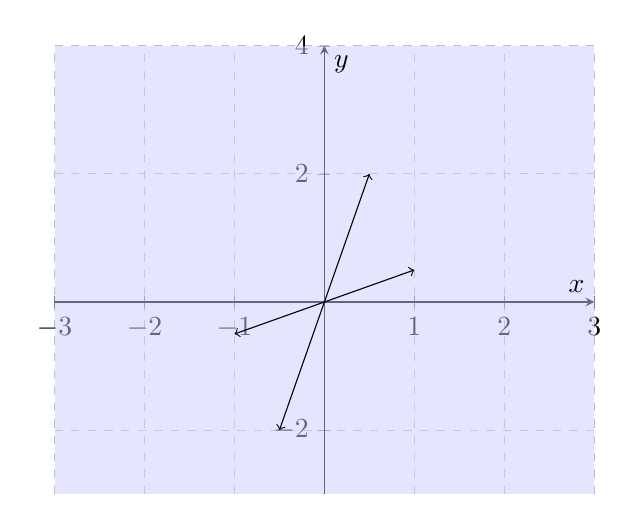
\begin{tikzpicture}
\begin{axis}[
    axis lines=middle,
    xlabel={$x$},
    ylabel={$y$},
    xmin=-3, xmax=3,
    ymin=-3, ymax=4,
    grid=major,
    grid style=dashed,
]

% Span area
\fill[blue!20, opacity=0.5] (axis cs:-3,-3) -- (axis cs:3,-3) -- (axis cs:3,4) -- (axis cs:-3,4) -- cycle;

% Some vectors in the span
\addplot[->, black] coordinates {(0,0) (1,0.5)};
\addplot[->, black] coordinates {(0,0) (-1,-0.5)};
\addplot[->, black] coordinates {(0,0) (0.5,2)};
\addplot[->, black] coordinates {(0,0) (-0.5,-2)};

\end{axis}
\end{tikzpicture}
\end{center}

This illustrates that all possible linear combinations of the columns \( \begin{bmatrix} 2 \\ -1 \end{bmatrix} \) and \( \begin{bmatrix} -1 \\ 2 \end{bmatrix} \) cover the entire 2D plane.


\subsection*{Matrix Formulation}
In matrix formulation we abandon scalar variables and numbers. Every entity is part of either a matrix or a vector as follows:

\begin{equation*}
    \begin{bmatrix}
        2 & -1 \\
        -1 & 2
    \end{bmatrix}
    \begin{bmatrix}
        x \\
        y
    \end{bmatrix}
    =
    \begin{bmatrix}
        0 \\
        3
    \end{bmatrix}
\end{equation*}


We assume we have $m$ equations and $n$ unknowns and can depict the matrix formulation as:

\[\mathbf{Ax} = \mathbf{b}\]

where \textbf{A} is a matrix of size $m\times n$ and \textbf{x} is a column vector of size $m\times 1$.


\subsection*{3D Matrix Example}

Consider the following system of three equations with three unknowns:
\begin{align}
    2x - y &= 0, \\
    -x + 2y - z &= -1, \\
    -3y + 4z &= 4.
\end{align}

This system can be written in matrix form \( \mathbf{A}\mathbf{x} = \mathbf{b} \) as:
\[
\mathbf{A} =
\begin{bmatrix}
    2 & -1 & 0 \\
    -1 & 2 & -1 \\
    0 & -3 & 4
\end{bmatrix},
\quad
\mathbf{b} =
\begin{bmatrix}
    0 \\
    -1 \\
    4
\end{bmatrix}.
\]

In row formulation, each row represents a plane in the 3D space. The solution of the system is where these three planes intersect. Visualising the solution in higher dimensions can be challenging.

% 3D planes intersection diagram
\begin{center}
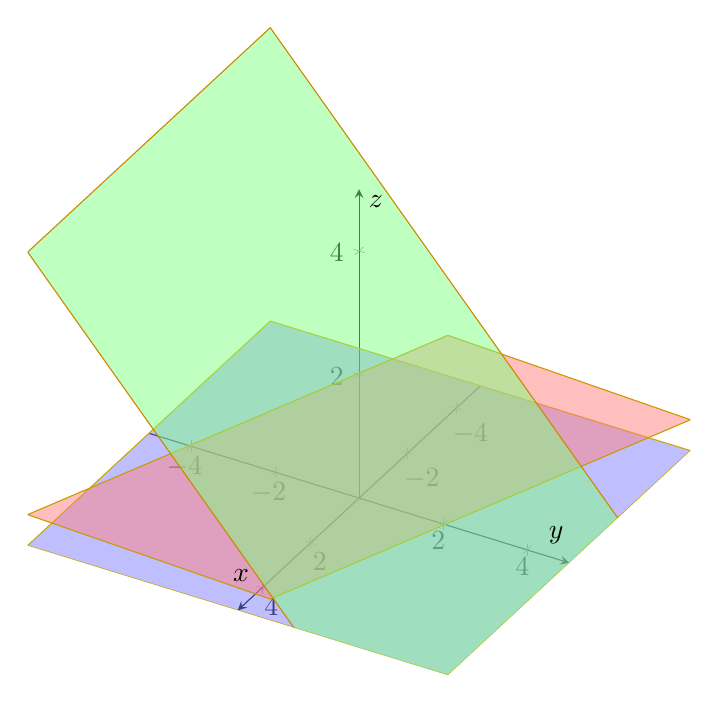
\begin{tikzpicture}
\begin{axis}[
    view={120}{40},
    axis lines=center,
    width=10cm,
    height=10cm,
    xmin=-5,
    xmax=5,
    ymin=-5,
    ymax=5,
    zmin=0,
    zmax=5,
    xlabel={$x$},
    ylabel={$y$},
    zlabel={$z$},
    grid=major,
    grid style={dashed, gray!30},
]

% Planes
\addplot3[surf, fill opacity=0.5, fill=blue!50, domain=-5:5, domain y=-5:5, samples=2, samples y=2] {0};
\addplot3[surf, fill opacity=0.5, fill=red!50, domain=-5:5, domain y=-5:5, samples=2, samples y=2] {(1/2)*x + (1/2)*y + 1/2};
\addplot3[surf, fill opacity=0.5, fill=green!50, domain=-5:5, domain y=-5:5, samples=2, samples y=2] {(-3/4)*y + 1};

\end{axis}
\end{tikzpicture}
\end{center}


In column formulation, the system is viewed as a combination of column vectors scaled by the unknowns:
\[
x \begin{bmatrix} 2 \\ -1 \\ 0 \end{bmatrix} +
y \begin{bmatrix} -1 \\ 2 \\ -3 \end{bmatrix} +
z \begin{bmatrix} 0 \\ -1 \\ 4 \end{bmatrix} =
\begin{bmatrix} 0 \\ -1 \\ 4 \end{bmatrix}.
\]



\begin{center}
\begin{tikzpicture}
\begin{axis}[
    width=10cm,
    height=10cm,
    view={135}{30},
    axis lines=center,
    xlabel={$x$},
    ylabel={$y$},
    zlabel={$z$},
    xmin=-5,
    xmax=5,
    ymin=-5,
    ymax=5,
    zmin=-5,
    zmax=5,
    grid=major,
    grid style={dashed, gray!30},
]

% Vector [2 -1 0]
\addplot3[->, blue, very thick] coordinates {(0,0,0) (2,-1,0)};
\node[anchor=south] at (axis cs:2,-1,0) {$\begin{bmatrix} 2 \\ -1 \\ 0 \end{bmatrix}$};

% Vector [-1 2 -3]
\addplot3[->, red, very thick] coordinates {(0,0,0) (-1,2,-3)};
\node[anchor=west] at (axis cs:-1,2,-3) {$\begin{bmatrix} -1 \\ 2 \\ -3 \end{bmatrix}$};

% Vector [0 -1 4]
\addplot3[->, green, very thick] coordinates {(0,0,0) (0,-1,4)};
\node[anchor=south] at (axis cs:0,-1,4) {$\begin{bmatrix} 0 \\ -1 \\ 4 \end{bmatrix}$};

\end{axis}
\end{tikzpicture}
\end{center}

The solution is the particular combination of column vectors that yield the right-hand side vector. For the given system, the solution is \(\mathbf{x} = \begin{bmatrix} 0 \\ 0 \\ 1 \end{bmatrix}\).
\begin{itemize}
    \item The solutions of a system of three equations with three unknowns lie within the 3D space. 
    \item A matrix \( \mathbf{A} \) is invertible if its column vectors are linearly independent, meaning they do not lie in the same plane. 
    \item If at least one column is a linear combination of the others, the matrix is not invertible, and the system may not have a unique solution for every \( \mathbf{b} \) in \( \mathbb{R}^3 \).
\end{itemize}



The concept of row and column formulations leads to the broader idea of vector spaces. Before delving deeper into vector spaces, it is essential to understand practical algorithms to solve systems of linear equations, such as Gaussian elimination.


\section{Gaussian Elimination}

Gaussian Elimination, also known as Row Reduction, is a systematic method for solving systems of linear equations. It involves performing operations on the rows of the augmented matrix of the system to obtain a row-echelon form, from which the solutions can easily be determined through back-substitution.

\subsection*{Example System}

Consider the system of linear equations:
\begin{align}
    x + 2y + z &= 2, \\
    3x + 8y + z &= 12, \\
    4y + z &= 2.
\end{align}

\subsection*{Row Reduction Process}

\textbf{Step 1:} Eliminate \( x \) from the second and third equations.

We multiply the first equation by 3 and subtract it from the second to eliminate \( x \):
\[
\begin{aligned}
    [2] - 3[1]: & \quad (3x + 8y + z) - 3( x + 2y + z) = 12 - 6, \\
    & \quad 2y - 2z = 6.
\end{aligned}
\]

\textbf{Step 2:} Multiply the first equation by 2 and subtract it from the third to eliminate \( x \):
\[
\begin{aligned}
    [3] - 2[1]: & \quad (4y + z) - 2( x + 2y + z)  = 2-2(2) , \\
    & \quad 5z = -10.
\end{aligned}
\]

\textbf{Step 3:} Now, we have a new system of equations:
\begin{align}
    x + 2y + z &= 2, \\
     2y - 2z &= 6, \\
    5z &= -10.
\end{align}

\textbf{Step 4:} We have achieved an upper triangular matrix.

\subsection*{Back-Substitution}

Once the matrix is in upper triangular form, we can find the solutions by back-substitution. The final form of the matrix and the solutions are:
\begin{align}
    x + 2y + z &= 2, \\
    2y - 2z &= 6, \\
    5z &= -10,
\end{align}

Since the system of equations is now in upper triangular form, we can solve the equations in reverse order. This method is straightforward because each equation can be solved for one variable at a time, starting from the last equation.\\


We start by solving the last equation for \( z \):
\begin{align*}
    5z &= -10 \\
    z &= \frac{-10}{5} \\
    z &= -2.
\end{align*}


Substituting \( z \) into the second equation, we solve for \( y \):
\begin{align*}
    2y - 2(-2) &= 6 \\
    2y + 4 &= 6 \\
    2y &= 6 - 4 \\
    2y &= 2 \\
    y &= \frac{2}{2} \\
    y &= 1.
\end{align*}


Finally, we substitute \( y \) and \( z \) back into the first equation to solve for \( x \):
\begin{align*}
    x + 2(1) - 2 &= 2 \\
    x + 2 - 2 &= 2 \\
    x &= 2 - 2 + 2 \\
    x &= 2.
\end{align*}



The solution to the system is:
\begin{align*}
    x &= 2, \\
    y &= 1, \\
    z &= -2.
\end{align*}





We solve the equations in reverse order because the system after elimination is triangular, allowing us to express each variable in terms of the subsequent ones.


\subsection*{Matrix Transformation}

The original matrix \( \mathbf{A} \) is:
\[
\mathbf{A} =
\begin{bmatrix}
    1 & 2 & 1 \\
    3 & 8 & 1 \\
    0 & 4 & 1
\end{bmatrix}.
\]

After applying the row operations \([2] - 3[1]\) and \([3] - 2[2]\), the matrix is transformed into:
\[
\mathbf{U} =
\begin{bmatrix}
    \boxeditem{1} & 2 & 1 \\
    0 & \boxeditem{2} & -2 \\
    0 & 0 & \boxeditem{5}
\end{bmatrix},
\]
where the elements in the diagonal of \( \mathbf{U} \) are called \textit{pivots}.

\subsection*{Column Transformation}

Similarly, the column vector \( \mathbf{b} \) is transformed alongside matrix \( \mathbf{A} \) as follows:
\[
\mathbf{b} =
\begin{bmatrix}
    2 \\
    12 \\
    2
\end{bmatrix}
\rightarrow
\begin{bmatrix}
    2 \\
    6 \\
    -10
\end{bmatrix}.
\]

\subsection*{Augmented Matrix}

It is often convenient to combine the matrix \( \mathbf{A} \) and the vector \( \mathbf{b} \) into an augmented matrix \( [ \mathbf{A} | \mathbf{b} ] \) and perform row operations on this combined matrix:
\[
[\mathbf{A}|\mathbf{b}] =
\left[
\begin{array}{ccc|c}
    1 & 2 & 1 & 2 \\
    3 & 8 & 1 & 12 \\
    0 & 4 & 1 & 2
\end{array}
\right]
\rightarrow
\left[
\begin{array}{ccc|c}
    1 & 2 & 1 & 2 \\
    0 & 2 & -2 & 6 \\
    0 & 0 & 5 & -10
\end{array}
\right].
\]

This augmented matrix represents the system after the row operations have been applied, and it is now ready for back-substitution to solve for the unknowns.



\section{LU Decomposition}

The process of Gaussian Elimination can be represented algebraically using matrices. Specifically, each elementary row operation can be performed by multiplying the matrix of coefficients by an \textit{elimination matrix}.

\subsection*{Transformation of Matrix A}

Consider the system of linear equations represented in matrix form by \( \mathbf{A}\mathbf{x} = \mathbf{b} \). The coefficient matrix \( \mathbf{A} \) is transformed through the elimination process as follows:

\[
\mathbf{A} =
\begin{bmatrix}
    1 & 2 & 1 \\
    3 & 8 & 1 \\
    0 & 4 & 1
\end{bmatrix}
\quad \underrightarrow{\text{[2] - 3[1]}}
\quad
\begin{bmatrix}
    1 & 2 & 1 \\
    0 & 2 & -2 \\
    0 & 4 & 1
\end{bmatrix}
\quad \underrightarrow{\text{[3] - 2[2]}}
\quad
\begin{bmatrix}
    1 & 2 & 1 \\
    0 & 2 & -2 \\
    0 & 0 & 5
\end{bmatrix} = \mathbf{U}
\]

\subsection*{Elimination Matrices}

Each step where a substitution of the form \([i] + c \times [j]\) is performed corresponds to multiplying the current matrix by an identity matrix with its \(i,j\) element replaced by \(c\). This special matrix is denoted \(E_{ij}\).

For instance, the first step \([2] - 3[1]\) can be represented by an elimination matrix \(E_{21}\):
\[
E_{21} =
\begin{bmatrix}
    1 & 0 & 0 \\
    -3 & 1 & 0 \\
    0 & 0 & 1
\end{bmatrix}
\]

\subsection*{Matrix Multiplication Representation}

The second step of elimination, \([3] - 2[2]\), can be represented as:
\[
E_{32} =
\begin{bmatrix}
    1 & 0 & 0 \\
    0 & 1 & 0 \\
    0 & -2 & 1
\end{bmatrix}
\]

Applying these elimination matrices to \( \mathbf{A} \) sequentially gives us \( \mathbf{U} \):
\[
E_{32}(E_{21}\mathbf{A}) = \mathbf{U}
\]
The brackets can be dropped due to the associative property of matrix multiplication, thus:
\[
E_{32}E_{21}\mathbf{A} = \mathbf{U}
\]

\subsection*{Inverses of Elimination Matrices}

The inverse of an elimination matrix \(E_{ij}\) is conveniently obtained by changing the sign of its non-zero off-diagonal element. For example:
\[
E_{21}^{-1} =
\begin{bmatrix}
    1 & 0 & 0 \\
    3 & 1 & 0 \\
    0 & 0 & 1
\end{bmatrix}
\quad \text{and} \quad
E_{32}^{-1} =
\begin{bmatrix}
    1 & 0 & 0 \\
    0 & 1 & 0 \\
    0 & 2 & 1
\end{bmatrix}
\]

The inverses of these matrices reverse the elimination steps, providing a method to return to the original matrix \( \mathbf{A} \).

LU decomposition is a method where a matrix \( \mathbf{A} \) is factorized into two matrices, \( \mathbf{L} \) and \( \mathbf{U} \), where \( \mathbf{L} \) is a lower triangular matrix and \( \mathbf{U} \) is an upper triangular matrix. This factorization is particularly useful for solving systems of equations, inverting matrices, and computing determinants.

\subsection*{Matrix Factorization}

The elimination process can be expressed as a sequence of matrix multiplications, transforming the original matrix \( \mathbf{A} \) into an upper triangular matrix \( \mathbf{U} \):
\[
E_{32}E_{21}\mathbf{A} = \mathbf{U}
\]

\subsection*{Inversion of Elimination Matrices}

By sequentially multiplying both sides from the left with the inverses of the elimination matrices in reverse order, we can express \( \mathbf{A} \) as:
\[
\mathbf{A} = E_{21}^{-1}E_{32}^{-1}\mathbf{U}
\]

\subsection*{Constructing Matrix L}

The product of the inverses of the elimination matrices gives us matrix \( \mathbf{L} \):
\[
\mathbf{L} = E_{21}^{-1}E_{32}^{-1} = \begin{bmatrix}
    1&0&0\\3&1&0\\0&2&1
\end{bmatrix}
\]
Matrix \( \mathbf{L} \) has the nice property that its elements below the diagonal are the multipliers used in the elimination process.

\subsection*{LU Decomposition}

Thus, matrix \( \mathbf{A} \) can be decomposed as:
\[
\mathbf{A} = \mathbf{L}\mathbf{U}
\]
This is the LU decomposition of \( \mathbf{A} \).

\subsection*{Permutation Matrix}

In the general case where row exchanges are required during the elimination process, we introduce a permutation matrix \( \mathbf{P} \). The PA = LU factorization incorporates these permutations:
\[
\mathbf{P}\mathbf{A} = \mathbf{L}\mathbf{U}
\]
A permutation matrix \( \mathbf{P} \) arises from the identity matrix if we reorder the rows to ensure that the pivot elements are non-zero.

\subsection*{Example of a Permutation Matrix}

For instance, if we need to swap rows 1 and 2 in matrix \( \mathbf{A} \) to get a non-zero pivot in the first position, the permutation matrix \( \mathbf{P}_{12} \) and the operation would look like this:
\[
\mathbf{P}_{12} =
\begin{bmatrix}
    0 & 1 & 0 \\
    1 & 0 & 0 \\
    0 & 0 & 1
\end{bmatrix}
\quad \text{and} \quad
\mathbf{P}_{12}\mathbf{A} =
\begin{bmatrix}
    0 & 1 & 0 \\
    1 & 0 & 0 \\
    0 & 0 & 1
\end{bmatrix}
\begin{bmatrix}
    1 & 2 & 1 \\
    3 & 8 & 1 \\
    0 & 4 & 1
\end{bmatrix}
=
\begin{bmatrix}
    3 & 8 & 1 \\
    1 & 2 & 1 \\
    0 & 4 & 1
\end{bmatrix}
\]

This reordering is essential to avoid dividing by zero when attempting to use that pivot to eliminate the variables in the column below.

\begin{definitionbox}{General LU Decomposition}

For any invertible matrix \( \mathbf{A} \), the LU decomposition with partial pivoting (where row exchanges are accounted for) can be expressed as:
\[
\mathbf{PA} = \mathbf{LU}
\]
Here, \( \mathbf{P} \) is the permutation matrix that records the row exchanges, \( \mathbf{L} \) is the product of the inverses of the elimination matrices (lower triangular), and \( \mathbf{U} \) is the resulting upper triangular matrix after applying Gaussian elimination.


The complete LU decomposition with a permutation matrix is thus represented as:
\[
\mathbf{A} = \mathbf{P}^{-1}\mathbf{L}\mathbf{U}
\]
It is important to note that \( \mathbf{P}^{-1} = \mathbf{P}^\mathsf{T} \) since permutation matrices are orthogonal.

\end{definitionbox}


\section{Vector Spaces, Inner Product and Norm}
We need to define a common framework to handle vectors in dimensions $\leq 3$ (geometry is useful) and in dimensions $> 3$.

\begin{definitionbox}{Vector Space}    
A vector space is a collection of vectors that form a nonempty set $E$ with two operations: addition and scalar multiplication that satisfy the following properties:

\begin{itemize}
    \item \textbf{Commutativity:} For all \( x, y \in E \), we have \( x + y = y + x \).
    \item \textbf{Associativity:} For all \( x, y, z \in E \), we have \( (x + y) + z = x + (y + z) \).
    \item \textbf{Distributivity:} For all \( x \in E \) and scalars \( \alpha, \beta \), we have \( (\alpha + \beta) x = \alpha x + \beta x \) and \( \alpha(x + y) = \alpha x + \alpha y \).
    \item \textbf{Existence of Inverses:} For every \( x, y \in E \) there exists \( z \in E \) such that \( x + z = y \).
    \item \textbf{Compatibility of Scalars and Multiplication:} For scalars \( \alpha, \beta \) and all \( x \in E \), we have \( \alpha(\beta x) = (\alpha\beta)x \).
    \item \textbf{Identity Element:} There exists an identity element \( 1 \) such that for every \( x \in E \), we have \( 1x = x \).
\end{itemize}
\end{definitionbox}

\begin{definitionbox}{Inner Product}
Let \( E \) be a complex vector space. A mapping \( \langle \cdot, \cdot \rangle \) from \( E \times E \rightarrow \mathbb{C} \) is called an inner product in \( E \) if for any \( x, y, z \in E \) and \( \alpha, \beta \in \mathbb{C} \) the following conditions are satisfied:
\begin{itemize}
    \item \textbf{Conjugate Symmetry:} \( \langle x, y \rangle = \overline{\langle y, x \rangle} \).
    \item \textbf{Linearity in the first argument:} \( \langle \alpha x + \beta y, z \rangle = \alpha \langle x, z \rangle + \beta \langle y, z \rangle \).
    \item \textbf{Positive-definiteness:} \( \langle x, x \rangle \geq 0 \) and \( \langle x, x \rangle = 0 \) implies \( x = 0 \).
\end{itemize}

In $\mathbb{C}$, the standard inner product between components of vectors $a, b \in \mathbb{C}^n$ can be written as 

\begin{equation}
\sum^n_{i=1}a_i \bar{b}_i    
\end{equation}

Where $\bar{b_i}$ is the complex conjugate of $b_i$.

\end{definitionbox}

\begin{definitionbox}{Norm}
It is always useful to be able to determine the size of an object, in the case of vector spaces this is achieved using the notion of ‘norm’.\\ 
A norm on a vector space \( E \) over \( \mathbb{C} \) (or \( \mathbb{R} \)) is a real-valued function with the following properties for any \( x, y \in E \) and \( \alpha \in \mathbb{C} \):
\begin{itemize}
    \item \textbf{Positive definiteness:} \( \|x\| \geq 0 \), and \( \|x\| = 0 \) if and only if \( x = 0 \).
    \item \textbf{Homogeneity Property:} \( \|\alpha x\| = |\alpha| \|x\| \).
    \item \textbf{Triangle Inequality:} \( \|x + y\| \leq \|x\| + \|y\| \).
\end{itemize}
Given the definition of inner product, we define the induced norm of a vector \( x \) as:
\[ \|x\|_2 = \sqrt{\langle x, x \rangle}  = \sqrt{\sum^n_{i=1}|x_i|^2}\]

The more general norm is defined as:
\[ \|x\|_p = \sqrt{\langle x, x \rangle}  = \left(\sum^n_{i=1}|x_i|^p\right) ^{\frac{1}{p}}\]

\end{definitionbox}


\subsection*{Examples of Vector Spaces}
\textbf{n-dimensional Vectors in \( \mathbb{R}^n \) or \( \mathbb{C}^n \)}\\
A vector is a set of scalars placed jointly in a vertical fashion (column vector).
\begin{itemize}
    \item A column vector of size \( n \) is denoted as \( \mathbf{x} = \begin{bmatrix} x_1 \\ x_2 \\ \vdots \\ x_n \end{bmatrix} \).
    \item The Hermitian transpose of \( \mathbf{x} \) is a row vector of size \( n \) denoted as \( \mathbf{x}^H = (x_1^* \ x_2^* \ \cdots \ x_n^*) \).
    \item Addition and product with a scalar are easily defined, while the inner product is: \( \langle \mathbf{x}, \mathbf{y} \rangle = \mathbf{y}^H \mathbf{x} = \sum_{i=1}^{n} x_i y_i^* \).
    \item Consequently, the induced norm is: \( \|\mathbf{x}\| = \sqrt{\langle \mathbf{x}, \mathbf{x} \rangle} = \left( \sum_{i=1}^{n} |x_i|^2 \right)^{1/2} \).
\end{itemize}
\textbf{Matrices of size \( m \times n \)}\\
The space of matrices of size \( m \times n \), that is, the space with elements \( A \in \mathbb{C}^{m \times n} \) includes:
\begin{itemize}
    \item Matrices are typically used to model linear equations but are more complex objects.
    \item The inner product of two matrices \( A, B \) is the element-by-element product: \( \langle A, B \rangle = \sum_{i,j} a_{i,j} b_{i,j}^* \).
    \item This leads to the induced norm (Frobenius norm): \( \|A\|_F = \sqrt{\sum_{i,j} |a_{i,j}|^2} \).
    \item More general norms: \( \|A\|_p = \sup_{\|x\|_p \neq 0} \frac{\|Ax\|_p}{\|x\|_p} \).
\end{itemize}

\newpage
\section*{On the Notion of the Norm}

\subsection*{Unit-norm Vectors for Different p-norms}

\begin{center}
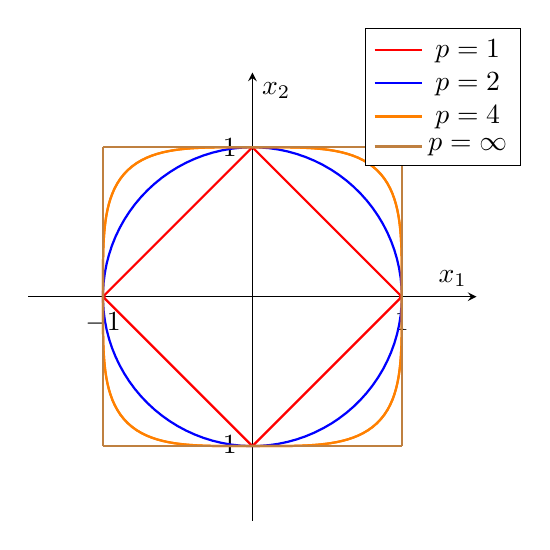
\begin{tikzpicture}
\begin{axis}[
    axis lines=middle,
    xlabel=\(x_1\),
    ylabel=\(x_2\),
    xmin=-1.5, xmax=1.5,
    ymin=-1.5, ymax=1.5,
    axis equal image,
    legend style={at={(1.1,1.1)},anchor=north east}
]

% Legend entries
\addlegendimage{red, thick}
\addlegendentry{\(p=1\)}
\addlegendimage{blue, thick}
\addlegendentry{\(p=2\)}
\addlegendimage{orange, thick}
\addlegendentry{\(p=4\)}
\addlegendimage{brown, thick}
\addlegendentry{\(p=\infty\)}

% 1-norm (diamond shape)
\addplot [red, thick, domain=-1:1, samples=100] ({1-abs(x)},x);
\addplot [red, thick, domain=-1:1, samples=100] ({-1+abs(x)},x);

% 2-norm (circle)
\addplot [blue, thick, domain=0:360, samples=100] ({cos(x)},{sin(x)});

% 4-norm
\addplot [orange, thick, domain=0:360, samples=100, variable=\t] 
    ({(cos(t)^(4) + sin(t)^(4))^(-1/4)*cos(t)}, {(cos(t)^(4) + sin(t)^(4))^(-1/4)*sin(t)});
\addplot [orange, thick, domain=0:360, samples=100, variable=\t] 
    ({-(cos(t)^(4) + sin(t)^(4))^(-1/4)*cos(t)}, {-(cos(t)^(4) + sin(t)^(4))^(-1/4)*sin(t)});

% Infinity norm (square)
\addplot [brown, thick, domain=-1:1] ({1},x);
\addplot [brown, thick, domain=-1:1] ({-1},x);
\addplot [brown, thick, domain=-1:1] (x,{1});
\addplot [brown, thick, domain=-1:1] (x,{-1});

\end{axis}
\end{tikzpicture}
\end{center}




Note: In this plot, the \( p \)-norm is defined for a unit vector \( x \) in \( \mathbb{R}^2 \) as \( \|x\|_p = \left( |x_1|^p + |x_2|^p \right)^{1/p} \), where \( p \) takes values of 1, 2, 4, \( \infty \), for the plotted shapes. Note that $p$ cannot take on non-integer values.


\section{Cauchy-Schwarz Inequality}


The Cauchy-Schwarz Inequality is a fundamental result in vector analysis which provides a bound for the absolute value of the inner product of two vectors.

\subsection{Introduction}
For all vectors \( \mathbf{x}, \mathbf{y} \) in an inner-product space, the following inequality holds:
\[ |\langle \mathbf{x}, \mathbf{y} \rangle| \leq \|\mathbf{x}\| \|\mathbf{y}\| \]


This inequality allows us to estimate the similarity of two vectors and to introduce the idea of direction. It is particularly useful in defining the angle between two vectors:
\[ \cos \theta = \frac{\langle \mathbf{x}, \mathbf{y} \rangle}{\|\mathbf{x}\| \|\mathbf{y}\|} \]

Two vectors are considered 'maximally' similar when one is a rescaled version of the other, and they are 'maximally' dissimilar, or orthogonal, when \( \theta = \frac{\pi}{2} \), that is, when \( \langle \mathbf{x}, \mathbf{y} \rangle = 0 \). If the vectors are orthogonal and their magnitudes are 1, they are called orthonormal.

\subsection{Proof of the Cauchy-Schwarz Inequality}

\textit{Sketch of the proof:}
Starting from the non-negativity of the norm, we have:
\[ 0 \leq \|\mathbf{x} - \alpha \mathbf{y}\|^2 = \langle \mathbf{x} - \alpha \mathbf{y}, \mathbf{x} - \alpha \mathbf{y} \rangle \]
Expanding the inner product, we get:
\[ = \|\mathbf{x}\|^2 - \langle \mathbf{x}, \alpha \mathbf{y} \rangle - \langle \alpha \mathbf{y}, \mathbf{x} \rangle + |\alpha|^2 \|\mathbf{y}\|^2 \]

Choosing \( \alpha = \frac{\langle \mathbf{x}, \mathbf{y} \rangle}{\|\mathbf{y}\|^2} \) and using the property that if \( c = \langle \mathbf{x}, \mathbf{y} \rangle \) then \( \langle \mathbf{y}, \mathbf{x} \rangle = c^* \), we obtain:
\[ 0 \leq \|\mathbf{x}\|^2 - \frac{|\langle \mathbf{x}, \mathbf{y} \rangle|^2}{\|\mathbf{y}\|^2} \]

Which simplifies to the Cauchy-Schwarz inequality:
\[ |\langle \mathbf{x}, \mathbf{y} \rangle|^2 \leq \|\mathbf{x}\|^2 \|\mathbf{y}\|^2 \]
And taking the square root of both sides gives us the final form of the inequality.

% \section{Linear Combination and Linear Independence}
\section{Linear Mappings, Basis and Dimension}

Let \( v_1, v_2, \ldots, v_n \) be vectors in a vector space of dimension \( n \). For scalar coefficients \( c_i \in \mathbb{R} \), the linear combination \( x \) can be expressed as:
    \[ x = c_1v_1 + c_2v_2 + \ldots + c_nv_n \]
    In matrix/vector form, this is represented as:
    \[
    x = \begin{bmatrix}
    v_{1,1} & v_{1,2} & \cdots & v_{1,n} \\
    v_{2,1} & v_{2,2} & \cdots & v_{2,n} \\
    \vdots & \vdots & \ddots & \vdots \\
    v_{n,1} & v_{n,2} & \cdots & v_{n,n}
    \end{bmatrix}
    \begin{bmatrix}
    c_1 \\
    c_2 \\
    \vdots \\
    c_n
    \end{bmatrix}
    \]

\begin{itemize}
    \item The vectors \( v_1, v_2, \ldots, v_n \) are \textbf{independent} if no linear combination of them gives the zero vector (except the trivial combination where all \( c_i = 0 \)).

    \item Two non-zero, non-parallel vectors in two-dimensional space are independent because no scalar multiples of one can be added to obtain the other.

    \item Considering three vectors in the two-dimensional space, they are \textbf{dependent} if there exists non-trivial scalars \( x_i \) such that:
    \[ x_1v_1 + x_2v_2 + x_3v_3 = 0 \]
    This means at least one vector is a linear combination of the others.
\end{itemize}

\subsection{Span}

\begin{definitionbox}{Span}
Let \( T \) be a set of vectors in a vector space \( E \). The \textbf{span} of \( T \), denoted \( \text{span}(T) \), is the set of all vectors that can be expressed as linear combinations of the vectors in \( T \). Formally, for \( V = \text{span}(T) \), any vector \( x \in V \) can be written as:
\[ x = \sum_{i} c_i v_i \]
where \( c_i \in \mathbb{R} \) and \( v_i \in T \). By construction, \( V \) is itself a vector space, and since \( V \subseteq E \), it is a subspace of \( E \).
\end{definitionbox}

\textbf{Example:} The span of two linearly independent vectors in \( \mathbb{R}^3 \) forms a plane, which is a subspace of \( \mathbb{R}^3 \).

\textit{Question:} Is the following plane a subspace as well?
\[ V = \{ x \in \mathbb{R}^3 : x_1 + x_2 + x_3 = 1 \} \]
To be a subspace, \( V \) must include the zero vector and be closed under addition and scalar multiplication. Since the sum of the components must equal 1, \( V \) does not include the zero vector and thus is not a subspace.

\subsection{Basis and Dimension}

\begin{definitionbox}{Vector Space Basis} A \textit{basis} for a vector space \( E \) is a set of vectors \( T \) that are linearly independent and span \( E \). The number of vectors in the basis is called the \textit{dimension} of \( E \).
\end{definitionbox}

\textbf{Example:} The standard basis for \( \mathbb{R}^n \) or \( \mathbb{C}^n \) consists of vectors \( e_i \), where each \( e_i \) has a 1 in the \( i \)-th position and 0s elsewhere. This basis is known as the \textit{canonical basis}.

When a basis also satisfies \( \langle v_i, v_j \rangle = 0 \) for \( i \neq j \), it is called an \textit{orthogonal basis}. If additionally \( \langle v_i, v_i \rangle = 1 \), it is an \textit{orthonormal basis}.

\textbf{Exercise:} Consider \( S = \{(1,2,\gamma)^T : \gamma \in \mathbb{R}\} \subset \mathbb{R}^3 \). The dimension of \( \text{span}(S) \) is 2, as \( S \) can be expressed as the span of \( \{(1,2,0)^T, (0,0,1)^T\} \), which are linearly independent.

\subsection{Orthogonal (Unitary) Matrices}

An \textit{orthonormal basis} of \( n \)-dimensional space can be formed into a matrix \( A \) that is orthogonal (unitary in the complex case). Such a matrix preserves the inner product and, consequently, the induced norm.

\subsubsection*{Properties of Orthogonal Matrices:}
\begin{itemize}
    \item For matrix \( A \) with orthonormal vectors as columns, \( A^HA = AA^H = I \), where \( I \) is the identity matrix, indicating \( A^H = A^{-1} \).
    \item Orthogonal matrices preserve the induced norm: \( \|Ax\|_2 = \|x\|_2 \).
    \item The process to orthogonalize a set of vectors is known as the \textit{Gram-Schmidt process}.
\end{itemize}

\subsubsection*{Examples of Orthogonal Matrices}

\textbf{Rotation Matrices:}
A rotation matrix in 2D is defined by \( Q = \begin{bmatrix} \cos \theta & -\sin \theta \\ \sin \theta & \cos \theta \end{bmatrix} \), which satisfies \( QQ^T = Q^TQ = I \).

\textbf{Permutation Matrices:}
Permutation matrices, such as \( P = \begin{bmatrix} 0 & 1 \\ 1 & 0 \end{bmatrix} \), reorder the rows of the identity matrix. They satisfy \( PQ = QP = I \).

\subsubsection*{Orthogonal Subspaces}

Extending the concept of orthogonality to subspaces requires every vector in one subspace to be orthogonal to every vector in the other subspace.

\begin{definitionbox}{Orthogonality} 
Two subspaces \( V \) and \( W \) of \( E \) are orthogonal if every vector \( v \in V \) is orthogonal to every vector \( w \in W \): \( \langle v, w \rangle = 0 \).
\end{definitionbox}

\begin{definitionbox}{Subspaces} 
The \textit{orthogonal complement} to a subspace \( V \subset E \), denoted \( V^\perp \), is the set of all vectors in \( E \) that are orthogonal to every vector in \( V \).
\end{definitionbox}


\section{Applications}
\subsection{Linear Mappings and Matrices}

\begin{itemize}
    \item We initially thought of matrices and vectors as a means to express linear equations in a compact form. Now, with a deeper understanding of vector spaces, we aim to interpret matrices more `geometrically'.
    \item Matrices facilitate the description of linear transformations between vector spaces. These transformations map vectors from one space, known as the domain, to another, known as the range.
\end{itemize}

\subsection{Understanding Matrix Operations through Linear Mappings}

Assume vector spaces \( X, Y \in \mathbb{R}^2 \), and consider a linear mapping represented by matrix \( A \) such that \( y = Ax \) with:

\[ A = \begin{bmatrix} \cos \theta & -\sin \theta \\ \sin \theta & \cos \theta \end{bmatrix} \]

This matrix \( A \) corresponds to a rotation by an angle \( \theta \) in the 2-dimensional Euclidean space.

\begin{itemize}
    \item To describe a rigid rotation in 3-D, we use rotation matrices that depend on the axis of rotation. For example, rotation about the \( z \)-axis by an angle \( \theta \) is represented by a similar trigonometric matrix with the addition of a third dimension.
    \item A 2-D rotation by \( 2\theta \) can be achieved by multiplying two matrices of rotation by \( \theta \), exploiting the property that matrix multiplication is associative.
    \item To invert a 2-D rotation by \( \theta \), we can either transpose the rotation matrix (since rotation matrices are orthogonal) or construct a new rotation matrix with angle \( -\theta \), effectively rotating in the opposite direction.
\end{itemize}




\subsection{Signal Processing}
Many important operations in signal processing can be describe using matrices.



\subsubsection*{Time-Reversal of Signals}
Given a discrete-time signal \( \mathbf{x} = (x_1, x_2, \ldots, x_n)^T \), its time-reversed version \( \mathbf{y}  = (x_n, \cdots, x_2, x_1)^T\) can be described by:
\[ \mathbf{y} = R\mathbf{x} \]
where \( R \) is the time-reversal matrix, a square matrix with 1's on its anti-diagonal and 0's elsewhere:
\[ R = \begin{bmatrix}
0 & \cdots & 0 & 1 \\
0& \cdots & 1 & 0 \\
\vdots  & \iddots & \vdots & \vdots \\
1 & \cdots & 0 & 0
\end{bmatrix} 
\quad R\mathbf{x} = \begin{bmatrix}
0 & \cdots & 0 & 1 \\
0& \cdots & 1 & 0 \\
\vdots  & \iddots & \vdots & \vdots \\
1 & \cdots & 0 & 0
\end{bmatrix} \begin{bmatrix}
    x_1 \\ x_2 \\ \vdots \\ x_n \\ 
\end{bmatrix} =\begin{bmatrix}
    x_n \\ \vdots \\ x_2 \\ x_1 \\ 
\end{bmatrix}   \]

\subsubsection*{Truncation of Signals}
Given a discrete-time signal \( \mathbf{x} = (x_1, x_2, \ldots, x_n)^T \), to truncate the last \( m-n \) terms of a signal with \(m<n\), use a truncation matrix \( T \) of size \( m \times n \) with 1's on the diagonal (the left part is a $mxm$ identity matrix) and 0's elsewhere:
\[ T = \begin{bmatrix}
1 & 0 & \cdots & 0 & 0&\cdots & 0 \\
0 & 1 & \cdots & 0 & 0&\cdots & 0 \\
\vdots & \vdots & \ddots & \vdots & \vdots&\cdots & \vdots \\
0 & 0 & \cdots & 1 & 0&\cdots & 0
\end{bmatrix} \]
Then \( \mathbf{y} = T\mathbf{x} \).

\[
\mathbf{y}=\begin{bmatrix}
1 & 0 & \cdots & 0 & 0&\cdots & 0 \\
0 & 1 & \cdots & 0 & 0&\cdots & 0 \\
\vdots & \vdots & \ddots & \vdots & \vdots&\cdots & \vdots \\
0 & 0 & \cdots & 1 & 0&\cdots & 0
\end{bmatrix} \begin{bmatrix}
    x_1 \\ x_2 \\ \vdots \\ x_m \\ x_{m+1} \\ \vdots \\ x_n
\end{bmatrix}= \begin{bmatrix}
    x_1 \\ x_2 \\ \vdots \\ x_m \\ 
\end{bmatrix} 
\]

\subsubsection*{Zero-Padding Operation}
Zero-padding a signal \( \mathbf{x} \) to length \( m > n \) can be done using an extension matrix \( E \) of size \( m \times n \). The zero-padded signal is \( \mathbf{y} = E\mathbf{x} \).
\[ E = \begin{bmatrix}
1 & 0 & \cdots & 0 \\
0 & 1 & \cdots & 0 \\
\vdots & \vdots & \ddots & \vdots \\
0 & 0 & \cdots & 1 \\
0 & 0 & \cdots & 0 \\
\vdots & \vdots & \ddots & \vdots \\
0 & 0 & \cdots & 0
\end{bmatrix}\quad E\mathbf{x}= \begin{bmatrix}
1 & 0 & \cdots & 0 \\
0 & 1 & \cdots & 0 \\
\vdots & \vdots & \ddots & \vdots \\
0 & 0 & \cdots & 1 \\
0 & 0 & \cdots & 0 \\
\vdots & \vdots & \ddots & \vdots \\
0 & 0 & \cdots & 0
\end{bmatrix} \begin{bmatrix}
    x_1 \\ x_2 \\ \vdots \\ x_n \\ 
\end{bmatrix} =\begin{bmatrix}
    x_1 \\ x_2 \\ \vdots \\ x_n \\ 0_{n+1} \\ \vdots \\ 0_m
\end{bmatrix}
\]

\subsubsection*{Permutation Operation}
A permutation matrix \( P \) rearranges the elements of a vector \( \mathbf{x} \). For example, to swap the first and second elements:
\[ P = \begin{bmatrix}
0 & 1 & 0 & \cdots & 0 \\
1 & 0 & 0 & \cdots & 0 \\
0 & 0 & 1 & \cdots & 0 \\
\vdots & \vdots & \vdots & \ddots & \vdots \\
0 & 0 & 0 & \cdots & 1
\end{bmatrix} \]
Applying \( P \) to \( \mathbf{x} \) yields the permuted vector. The permutation matrix has a single `1' in every row and column.

\subsubsection*{Differentiation of Polynomials}
We can represent a general polynomial of degree $n$ with a $n+1$-dimensional vector. For example, $p(x) = c_0 + c_1x + c_2x^2$ can be represented as $\mathbf{p} = \begin{bmatrix}
    c_0\\c_1\\c_2
\end{bmatrix}$. The derivative of $p(x)$ is $p'(x) = c_1 + 2c_2x$ represented as  $\mathbf{p'} = \begin{bmatrix}
    c_1\\2c_2\\0
\end{bmatrix}.$ We can express the differentiation using matrix $D_2 = \begin{bmatrix}
    0&1&0\\0&0&2\\0&0&0
\end{bmatrix}$ that satisfies $D_2 \mathbf{p}=\mathbf{p'}$

For differentiating a polynomial of degree \( d \), represented by a vector of its coefficients \( \mathbf{a} \), the differentiation matrix \( D \) is:
\[ D = \begin{bmatrix}
0 & 1 & 0 & \cdots & 0 \\
0 & 0 & 2 & \cdots & 0 \\
\vdots & \vdots & \vdots & \ddots & \vdots \\
0 & 0 & 0 & \cdots & d \\
0 & 0 & 0 & \cdots & 0
\end{bmatrix} \]
The derivative \( \mathbf{a}' \) is obtained by \( \mathbf{a}' = D\mathbf{a} \).

\subsection{Circulant Matrices}

Circulant matrices are a special class of matrices that play an important role in various applications, including signal processing and time series analysis. They are defined by the property that each row is a cyclic shift of the one above it.
\subsubsection*{Shifting a Vector}

Assume we have a vector \( \mathbf{x} = (x_1, x_2, \ldots, x_n)^T \). To shift this vector by one unit to the right (or when looking vertically, one unit to the bottom), we can use a permutation matrix \( P \). For \( n = 4 \), the matrix and the shifted vector are given by:

\[
P = \begin{bmatrix}
0 & 0 & 0 & 1 \\
1 & 0 & 0 & 0 \\
0 & 1 & 0 & 0 \\
0 & 0 & 1 & 0
\end{bmatrix}, \quad
P\mathbf{x} = \begin{bmatrix}
0 & 0 & 0 & 1 \\
1 & 0 & 0 & 0 \\
0 & 1 & 0 & 0 \\
0 & 0 & 1 & 0
\end{bmatrix}  \begin{bmatrix}
x_1 \\
x_2 \\
x_3 \\
x_4
\end{bmatrix} =\begin{bmatrix}
x_4 \\
x_1 \\
x_2 \\
x_3
\end{bmatrix}
\]

Multiplying \( \mathbf{x} \) by \( P^2 \) and \( P^3 \) will cyclically shift the vector by 2 and 3 units, respectively.

\subsubsection*{Constructing a Circulant Matrix}

A circulant matrix \( C \) is constructed as a linear combination of identity matrix \( I \) and powers of the permutation matrix \( P \). For \( n = 4 \), \( C \) can be expressed as:

\[
C = c_0I + c_1P + c_2P^2 + c_3P^3 = \begin{bmatrix}
c_0 & c_3 & c_2 & c_1 \\
c_1 & c_0 & c_3 & c_2 \\
c_2 & c_1 & c_0 & c_3 \\
c_3 & c_2 & c_1 & c_0
\end{bmatrix}
\]

Importantly, this structure enables \( C \) to perform a filtering operation, where the \( c_i \)'s represent the filter coefficients.\\

\[
\mathbf{y} = C\mathbf{x}
\]

The action of \( C \) can be thought of as applying a filter to the signal \( \mathbf{x} \), where the filter characteristics are determined by the coefficients \( c_i \). More generally, it can be defined as:

\begin{equation}
C = \begin{bmatrix} 
c_0 & c_{n-1} & \cdots & c_2 & c_1 \\ 
c_1 & c_0 & c_{n-1} & \cdots & c_2 \\ 
\vdots & c_1 & c_0 & \ddots & \vdots \\ 
c_{n-2} & \cdots & \ddots & \ddots & c_{n-1} \\ 
c_{n-1} & c_{n-2} & \cdots & c_1 & c_0 
\end{bmatrix}
\end{equation}

Convolution is a process of combining two sequences to produce a third sequence, which is the modification or filtering of an original signal.

\subsubsection*{Convolution through Circulant Matrices}
Multiplying a circulant matrix \(C\) by a vector \(x\) is equivalent to convolving the first row of \(C\) with \(x\). For example:

\begin{align*}
C &= \begin{bmatrix} c_0 & c_1 & c_2 \\ c_2 & c_0 & c_1 \\ c_1 & c_2 & c_0 \end{bmatrix} \\
\textbf{x} &= \begin{bmatrix} x_0 \\ x_1 \\ x_2 \end{bmatrix} \\
\textbf{y} &= C\textbf{x} = \begin{bmatrix} 
c_0x_0 + c_1x_1 + c_2x_2 \\ 
c_2x_0 + c_0x_1 + c_1x_2 \\ 
c_1x_0 + c_2x_1 + c_0x_2 
\end{bmatrix}
\end{align*}

\subsection{Discrete-Time Convolution and FIR Filters}
Discrete-time convolution is a fundamental operation in signal processing where a filter with an impulse response \( h_k \) is applied to an input signal \( x_n \) to produce an output signal \( y_n \). This process is mathematically expressed as:
\begin{equation*}
    y_n = \sum_k h_k x_{n-k}
\end{equation*}
The operation involves 'sliding' the filter \( h_k \) over the input sequence \( x_n \) and summing the products of \( h_k \) and \( x_{n-k} \) for each \( n \). It is assumed that the filter has a finite impulse response (FIR), meaning that \( h_k \neq 0 \) only for a finite number of samples \( k \), and that the input sequence also has finite duration where \( n > K \). \\

Under such conditions, convolution is a linear mapping from $\mathbb{R}^n$ to $\mathbb{R}^m$:

\[\mathbf{y} = A\mathbf{x}\]


Convolution can be represented as a linear operation using matrices. For FIR filters, this operation is typically represented by a Toeplitz matrix \( A \), which has constant values along its diagonals. The matrix multiplication \( y = Ax \) can then be used to perform the convolution, where \( A \) is structured such that each row is a shifted version of the impulse response \( h_k \). \\

$A \in \mathbb{R}^{m\times n}$ is generally represented as:

\[
y=h*x=A\mathbf{x} = \begin{bmatrix}
h_0&0&\cdots&0&0\\
h_1&h_0&&\vdots&\vdots\\
h_2&h_1&\cdots&0&0\\
\vdots&h_2&\cdots&h_0&0\\
h_{K-2}&\vdots&\ddots&h_1&h_0\\
h_{K-1}&h_{K-2}&&\vdots&h_1\\
0&h_{K-1}&\ddots&h_{K-3}&\vdots
\\0&0&\cdots&h_{K-2}&h_{K-3}\\
\vdots&\vdots&&h_{K-1}&h_{K-2}\\
0&0&0&\cdots&h_{K-1}\\
\end{bmatrix}\begin{bmatrix}x_1\\x_2\\x_3\\\vdots\\x_n\end{bmatrix}
\]
% \[
% A=\begin{bmatrix}
% h_0&0&\cdots&\cdots&\cdots&0\\
% h_1&h_0&\cdots&\cdots&\cdots&\vdots\\
% \vdots&h_1&\ddots&\ddots&\ddots&0\\
% h_{K-1}&\vdots&\ddots&\ddots&\vdots&\vdots\\
% 0&h_{K-1}&\vdots&\vdots&\vdots&0\\
% \vdots&\ddots&\ddots&\ddots&\ddots&\vdots\\
% 0&\ddots&\ddots&\ddots&h_1&h_0\\
% 0&\ddots&\ddots&\ddots&h_2&h_1\\
% \vdots&\ddots&\ddots&\ddots&\ddots&\vdots\\
% 0&\cdots&\cdots&\cdots&0&h_{K-1}
% \end{bmatrix}
% \]

% So for a convolution (clearer version of the matrix):

% \[
% y=h*x=A\mathbf{x} = \begin{bmatrix}h_0&0&\cdots&0&0\\h_1&h_2&&\vdots&\vdots\\h_2&h_1&\cdots&0&0\\\vdots&h_2&\cdots&h_0&0\\h_{K-2}&\vdots&\ddots&h_1&h_0\\h_{K-1}&h_{K-2}&&\vdots&h_1\\0&h_{K-1}&\ddots&h_{K-3}&\vdots\\0&0&\cdots&h_{K-2}&h_{K-3}\\\vdots&\vdots&&h_{K-1}&h_{K-2}\\0&0&0&\cdots&h_{K-1}\\\end{bmatrix}\begin{bmatrix}x_1\\x_2\\x_3\\\vdots\\x_n\end{bmatrix}
% \]

\subsection{Linear and Circular Convolution}
The difference between linear and circular convolution is distinguished by how the input signal is treated. Linear convolution, which uses a Toeplitz matrix, assumes the input \( x \) is non-periodic and has a length \( m = n + K - 1 \) to accommodate the length of the convolved signal. In contrast, circular convolution assumes the input signal is periodic and wraps around the end of the signal back to the start. This is modeled using a circulant matrix \( A \), which is a special case of the Toeplitz matrix where the end of the impulse response wraps around to the beginning of the next row.


\begin{figure}[H]
    \centering
    \includegraphics[width=0.5\linewidth]{img/linear_conv.png}
    \caption{A \(\in \mathbb{R}^{m \times n}\) with \(m = n + K - 1\) models the linear convolution.
}
    \label{fig:linear_conv}
\end{figure}


\begin{figure}[H]
    \centering
    \includegraphics[width=1\linewidth]{img/cir_conv.png}
    \caption{If we want \(A\) to be square, we may assume that \(x \in \mathbb{R}^n\) is periodic outside the interval of observation. In this case \(A\) is a `circulant' matrix and models the circulant convolution.}
    \label{fig:circ-conv}
\end{figure}

\subsubsection*{Example of Linear and Circulant Convolution}
Assume you want to implement a discrete-time version of the derivative \( y(t) = \frac{dx(t)}{dt} \). The natural way to do it is by taking finite differences of the incoming sequence: \( y_n = x_n - x_{n-1} \). This is achieved by filtering with \( h_k = [1, -1] \):

\[
y_n = \sum_k h_k x_{n-k}
\]

In the case of linear convolution, the linear mapping is described by the \( (n + 1) \times n \) matrix:

\[
\mathbf{A} = \begin{bmatrix}
h_0&0&\cdots&0&0\\
h_1&h_0&&\vdots&\vdots\\
h_2&h_1&\cdots&0&0\\
\vdots&h_2&\cdots&h_0&0\\
h_{K-2}&\vdots&\ddots&h_1&h_0\\
h_{K-1}&h_{K-2}&&\vdots&h_1\\
0&h_{K-1}&\ddots&h_{K-3}&\vdots
\\0&0&\cdots&h_{K-2}&h_{K-3}\\
\vdots&\vdots&&h_{K-1}&h_{K-2}\\
0&0&0&\cdots&h_{K-1}\\
\end{bmatrix}=\begin{bmatrix}
1 & 0 & 0 & \cdots &0&0\\
-1& 1 & 0& \cdots &0&0\\
0 & -1& 1 & \cdots &0&0\\
\vdots&\vdots&\ddots& \ddots&\vdots&\vdots\\
0 & 0 & \cdots  & -1& 1 & 0\\
0 & 0 & \cdots  & 0 & -1 & 1 \\
0 & 0 & \cdots  & 0 &  0 & -1
\end{bmatrix}
\]

In the case of circulant convolution, the linear mapping is described by the \( n \times n \) matrix:

\[
\mathbf{A} = \begin{bmatrix}
1 & 0 & 0 & \cdots &0&0\\
-1& 1 & 0& \cdots &0&0\\
0 & -1& 1 & \cdots &0&0\\
\vdots&\vdots&\ddots& \ddots&\vdots&\vdots\\
0 & 0 & \cdots  & -1& 1 & 0\\
0 & 0 & \cdots  & 0 & -1 & 1 \\
\end{bmatrix}
\]




\subsection{Discrete-time Fourier Transform}

The discrete Fourier Transform (DFT) is a linear mapping and can be described by a matrix. Recall that given the finite-length sequence: $x_0, x_1, \cdots, x_{N-1}$ the DF is given by:

\[X_{r}=\sum_{n=0}^{N-1}x_{n}e^{-j2\pi\frac{rn}{N}}\quad r=0,1,...N-1\]

\[\begin{bmatrix}X_0\\X_1\\\vdots\\X_{N-1}\end{bmatrix}=\begin{bmatrix}1&1&1&\cdots&1\\1&e^{-j\frac{2\pi}N}&e^{-j\frac{4\pi}N}&\vdots&e^{-j2\pi\frac{N-1}N}\\1&e^{-j\frac{4\pi}N}&\vdots&\vdots&\vdots\\\vdots&\vdots&\vdots&\vdots&e^{-j2\pi\frac{(N-2)(N-2)}N}\\1&e^{-j2\pi\frac{N-1}N}&\cdots&e^{-j2\pi\frac{(N-1)(N-2)}N}&e^{-j2\pi\frac{(N-1)(N-1)}N}\end{bmatrix}\begin{bmatrix}x_0\\x_1\\\vdots\\\vdots\\x_{N-1}\end{bmatrix}\]





\section{Range and Null Space}

\subsection{Introduction}

Consider the linear transformation \( \mathbf{X} \rightarrow \mathbf{Y} \) represented by the matrix

\[ A = \begin{pmatrix}
1 & 2 & 0 \\
1 & 2 & 0 \\
0 & 0 & 1 \\
\end{pmatrix} \]

The matrix \( A \) maps vectors from \( \mathbb{R}^3 \) to \( \mathbb{R}^3 \). However, the first two rows of \( A \) are identical, indicating that all vectors \( \mathbf{X} \) are mapped to a plane in \( \mathbb{R}^3 \). This redundancy suggests that the mapping is not one-to-one since different vectors in \( \mathbb{R}^3 \) could result in the same vector in \( \mathbb{R}^3 \) after transformation. Consequently, we infer that the transformation is not invertible.\\

In an intuitive sense, the elements have been collapse into a 2D plane despite the mapping being from \( \mathbb{R}^3 \) to \( \mathbb{R}^3 \). Since information `is lost' after transformation, we feel that this mapping is not invertible.\\

The concepts of range space (or column space) and null space (or kernel) of \( A \) help to formalise this intuition. The range space is the set of all possible outputs \( \mathbf{Y} \), which, in this case, is a plane in \( \mathbb{R}^3 \). The null space is the set of all vectors \( \mathbf{X} \) that map to the zero vector in \( \mathbb{R}^3 \), indicating the loss of information and confirming the non-invertibility of the transformation.


\begin{figure}[H]
\begin{center}
\tdplotsetmaincoords{70}{110} % to set the orientation of the 3D plot
\begin{tikzpicture}[scale=1,tdplot_main_coords,>=stealth]

% Left R^3 axes
\draw[->] (0,0,0) -- (3,0,0) node[anchor=north east]{$y_1$};
\draw[->] (0,0,0) -- (0,3,0) node[anchor=north west]{$y_2$};
\draw[->] (0,0,0) -- (0,0,3) node[anchor=south]{$y_3$};

% Vectors in left R^3
\draw[->,thick,green] (0,0,0) -- (1,1,0);
\draw[->,thick,orange] (0,0,0) -- (2,2,0);
\draw[->,thick,purple] (0,0,0) -- (0,0,1);

% Plane 2x-y=0 (range space)
\fill[blue,opacity=0.3] (0,0,0) -- (3,3,0) -- (3,3,3) -- (0,0,3) -- cycle;
\node[anchor=south] at (3,4.2,0) {Range space};

% Right R^3 axes
\draw[->] (5,0,0) -- (8,0,0) node[anchor=north east]{$x_1$};
\draw[->] (5,0,0) -- (5,3,0) node[anchor=west]{$x_2$};
\draw[->] (5,0,0) -- (5,0,3) node[anchor=south]{$x_3$};

% Vectors in right R^3
\draw[->,thick,green] (5,0,0) -- (6,0,0);
\draw[->,thick,orange] (5,0,0) -- (5,1,0);
\draw[->,thick,purple] (5,0,0) -- (5,0,1);

% Connecting arrows
\draw[<->,dashed] (1,1,0) -- (6,0,0);
\draw[<->,dashed] (2,2,0) -- (5,1,0);
\draw[<->,dashed] (0,0,1) -- (5,0,1);

% Null space line
\draw[dotted, thick, red] (9,-2,0) -- (1,2,0);
\node[anchor=north] at (7,-2,0) {Null space};

\end{tikzpicture}
\end{center}
\caption{Visualised mapping}
\label{fig:mapping_linear_transform}

\end{figure}

We observe:
\begin{itemize}
    \item The columns of \textbf{A} are linearly dependent.
    \item The first and third column are only independent columns.
    \item The plane where all the vectors \textbf{x} were collapsing to is the $\text{span}\{ \begin{pmatrix}1\\1\\0\end{pmatrix},\begin{pmatrix}0\\0\\1\end{pmatrix}\}$, the range of the matrix
    \item We note that if $\mathbf{x} = \begin{pmatrix}
        2\\-1\\0
    \end{pmatrix}$ then $\mathbf{Ax} = 0$, so $\mathbf{x} = \begin{pmatrix}
        2\\-1\\0
    \end{pmatrix}$ is in the null space of \textbf{A} and is orthogonal to the range space.
\end{itemize}

\begin{definitionbox}{Range and Null Space}
Let \( A: X \rightarrow Y \) be a linear transformation. The \textbf{range space} \( \mathcal{R}(A) \) is the set of values in \( Y \) that are reached from \( X \) by applying \( A \):
\[ \mathcal{R}(A) = \{y = Ax : x \in X\} \]
The \textbf{null space} \( \mathcal{N}(A) \) is the set of values in \( X \) that are transformed to \( 0 \) by \( A \):
\[ \mathcal{N}(A) = \{x \in X : Ax = 0\} \]

Let \( A \) be an \( m \times n \) matrix which we regard as a linear operator and which we write as follows:
\[ A = [v_1 \quad v_2 \quad \ldots \quad v_n] \]
then a vector \( x \in \mathbb{R}^n \) is transformed as:
\[ Ax = x_1v_1 + x_2v_2 + \ldots + x_nv_n \]
which is a linear combination of the columns of \( A \).\\

This means that the range can be expressed as
\[ \mathcal{R}(A) = \text{span}\{v_1, v_2, \ldots, v_n\} \]
and corresponds to the column space of \( A \). Moreover, the number of linear independent columns of \( A \), which by definition is also the rank of \( A \), corresponds to the dimension of \( \mathcal{R}(A) \).\\

The null space of \( A \) is also a subspace and its dimension is \( n - \text{rank}(A) \).\\

When the dimension of \( \mathcal{N}(A) > 0 \) then the mapping is not invertible. Assume that \( An_1 = 0 \) and that \( y_1 = Ax_1 \), then, given \( x_2 = x_1 + n_1 \), we have that \( Ax_2 = Ax_1 + An_1 = Ax_1 = y_1 \). Therefore given \( y_1 \) it is not possible to know whether it is due to \( x_1 \) or \( x_2 \).\\

\textbf{Sketch of the Proof:}
\begin{itemize}
  \item Remember that when we compute \( Ax \) we are effectively taking a linear combination of the columns of \( A \)
  \item Assume for the sake of argument that \( \text{rank}(A) = n - 2 \), this means that given \( n - 2 \) columns of \( A \), the other two columns can be obtained with proper linear combinations of the linearly independent \( n - 2 \) columns.
  \item Therefore there are two linearly independent vectors \( x_1 \) and \( x_2 \) such that \( Ax_1 = Ax_2 = 0 \)
  \item Moreover any linear combination of \( x_1 \) and \( x_2 \) is also in the null space of \( A \), therefore that space has dimension 2.
\end{itemize}

Assume that \( A \) models a linear mapping from \( \mathbb{C}^n \) to \( \mathbb{C}^n \) and that its null space is non-trivial (i.e., it has dimension larger than 0 or \( \text{rank}(A) < n \)) then the mapping is not invertible or in other words the matrix \( A \) does not have an inverse.\\

In this case we call \( A \) a \textbf{singular matrix}.
    
\end{definitionbox}

\subsection{Computing the Nullspace}
\begin{itemize}
    \item Get row-echelon form (staircase) \textbf{u}
    \item Identify pivot columns and free columns
    \item To find nullspace solve $\textbf{ux} =0$
    \item Find the solution expressed as a function of free variables that correspond to the pivot columns position    
\end{itemize}

Let's consider matrix \( A \) and calculate its null space.

Given the matrix:
\[ A = \begin{bmatrix}
1 & 2 & 2 & 2 \\
2 & 4 & 6 & 8 \\
3 & 6 & 8 & 10
\end{bmatrix} \]

By applying elimination, we obtained the matrix \( u \):
\[ u = \left[ \begin{array}{cccc}
\color{red}1 & \color{red}2 & \color{blue}2 & \color{blue}2 \\
0 & 0 & \color{blue}2 & \color{blue}4 \\
0 & 0 & 0 & 0
\end{array} \right] \]

The matrix \( u \) contains two \textcolor{red}{pivot columns} shown in red and two \textcolor{blue}{free columns} shown in blue.

To calculate the null space \( \mathcal{N}(A) \), we need to solve the system \( Ax = 0 \). The system \( Ax = 0 \) is equivalent to \( ux = 0 \) which can be written as:
\[ ux = \begin{bmatrix}
\color{red}1 & \color{blue}2 & \color{red}2 & \color{blue}2 \\
0 & 0 & \color{red}2 & \color{blue}4 \\
0 & 0 & 0 & 0
\end{bmatrix}
\begin{bmatrix}
x_1 \\
x_2 \\
x_3 \\
x_4
\end{bmatrix} = 0 \]

Using row formulation, we obtain:
\begin{align*}
x_1 + 2x_2 + 2x_3 + 2x_4 &= 0 \\
2x_3 + 4x_4 &= 0 \\
\end{align*}

The solution of the above system is of the form:
\[
\begin{bmatrix}
x_1 \\
x_2 \\
x_3 \\
x_4
\end{bmatrix} = 
\begin{bmatrix}
-2x_2 + 2x_4 \\
x_2 \\
-2x_4 \\
x_4
\end{bmatrix} = x_2
\begin{bmatrix}
-2 \\
1 \\
0 \\
0
\end{bmatrix} + x_4
\begin{bmatrix}
2 \\
0 \\
-2 \\
1
\end{bmatrix}
\]

Variables \( x_2 \) and \( x_4 \) can take any values (free variables).\\

By assigning the value of 1 to a particular free variable and the value of 0 to the rest of the free variables, we obtain a so-called \textbf{special solution}.

The first special solution is obtained for \( x_2 = 1, x_4 = 0 \) and is:
\[
\begin{bmatrix}
-2 \\
1 \\
0 \\
0
\end{bmatrix}
\]

The second special solution is obtained for \( x_2 = 0, x_4 = 1 \) and is:
\[
\begin{bmatrix}
2 \\
0 \\
-2 \\
1
\end{bmatrix}
\]

The null space is the linear combination of the special solutions:
\[
\begin{bmatrix}
x_1 \\
x_2 \\
x_3 \\
x_4
\end{bmatrix} = c
\begin{bmatrix}
-2 \\
1 \\
0 \\
0
\end{bmatrix} + d
\begin{bmatrix}
2 \\
0 \\
-2 \\
1
\end{bmatrix}
\]

\section*{Range and Null Space for Linear Filtering}

\begin{itemize}
    \item Convolution and linear filtering are fundamental operations in signal processing. They can be algebraically represented using matrices.
    \item For linear systems, the convolution operation can be described by the Toeplitz matrix \( A \) through the equation \( y = Ax \), where \( y \) is the output signal and \( x \) is the input signal.
    \item The process of deconvolution aims to reverse this operation, attempting to retrieve the input signal \( x \) from the output signal \( y \).
    \item Understanding the range (or column space) and the null space of the matrix \( A \) is crucial because it informs us about the invertibility of the convolution operation. Specifically, the range tells us what outputs are possible, and the null space indicates if there are any inputs that could yield a zero output.
    \item \textbf{Claim} (without proof): If matrix \( A \) represents a linear convolution, then the null space is typically trivial, meaning there are no non-zero inputs that give a zero output. This is in contrast to circulant convolution, where the null space is generally non-trivial, allowing for the existence of non-zero inputs that do produce a zero output.
    \item \textbf{Example}: In the context of finite difference operations, consider a vector \( x \) consisting entirely of ones. For a circulant convolution matrix \( A \), this particular \( x \) would lie in the null space of \( A \), meaning that applying \( A \) to \( x \) would yield a zero vector, which signifies that no change would be detected in the signal.
\end{itemize}